\section{镜像下降}
\label{sec:feas-mirror}

在预算例中，把第三个项目的份额从$0.01$变到$0.02$和从$0.50$变到$0.51$，欧氏距离相同。可是前者把这个项目的份额翻了一倍，后者几乎没有变化。对比例这样的量，有没有一把更合适的尺子？本节回答这个问题：把投影梯度中的欧氏距离换成由凸势函数决定的代价，然后在单纯形上算出具体的公式。

\subsection{Bregman距离}
\label{sec:feas-bregman}

欧氏距离的平方可以看成是$\tfrac12\lVert\bm{x}\rVert_2^2$这个碗与它的切平面之间的高度差。换一只碗，就换了一把尺子。

\paragraph{定义}
设$h$是凸函数，在点$\bm{x}$可微。把$h$在$\bm{x}$处的切平面延伸到$\bm{u}$，势函数实际值高出切平面的量就是我们要的代价。

\begin{definition}[Bregman距离]
\label{def:feas-bregman}
设$h$是凸函数，在$\bm{x}$处可微，$\bm{u}\in\operatorname{dom}h$。称
\begin{equation}
 D_h(\bm{u},\bm{x})=h(\bm{u})-h(\bm{x})-\langle\nabla h(\bm{x}),\bm{u}-\bm{x}\rangle
 \label{eq:feas-bregman}
\end{equation}
为\term{势函数}$h$生成的\term{Bregman距离}（Bregman distance）。
\end{definition}

本节的$h$是势函数，与等式约束无关。由凸性，切平面不高于$h$，所以$D_h(\bm{u},\bm{x})\geq0$；若$h$严格凸，等号只在$\bm{u}=\bm{x}$时成立。

取$h(\bm{x})=\tfrac12\lVert\bm{x}\rVert_2^2$，代入式~\eqref{eq:feas-bregman}，得到
\[
 D_h(\bm{u},\bm{x})=\tfrac12\lVert\bm{u}\rVert_2^2-\tfrac12\lVert\bm{x}\rVert_2^2-\langle\bm{x},\bm{u}-\bm{x}\rangle=\tfrac12\lVert\bm{u}-\bm{x}\rVert_2^2.
\]
这时恰好是欧氏距离平方的一半。

\paragraph{不是真正的距离}
名字里虽有“距离”，$D_h$通常不对称，也不满足三角不等式。图~\ref{fig:feas-bregman-tangent}对比了两种势函数：抛物线上两条竖线段长度相等，$x\ln x$的曲线上两条竖线段长度不同。

\begin{BookInlineFigure}
  \centering
  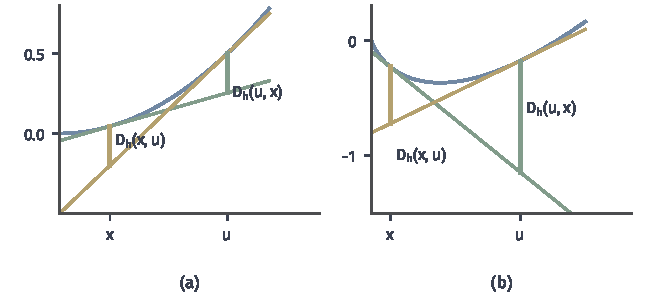
\includegraphics[width=112mm]{figures/05-optimization/06-constrained-optimization/matplotlib/feas-bregman-tangent/figure.pdf}
  \caption{Bregman距离是势函数高出切线的量。蓝线是势函数，绿线和黄线分别是$x$和$u$处的切线，同色竖线段分别是$D_h(u,x)$和$D_h(x,u)$。(a)$h(t)=t^2/2$，两段等长。(b)$h(t)=t\ln t$，$x=0.1$，$u=0.8$，两段不等长。}
  \label{fig:feas-bregman-tangent}
\end{BookInlineFigure}

用一个可手算的例子来看。取$h(\bm{x})=\sum_ix_i\ln x_i$和两个坐标和为一的点
\[
 \bm{u}=(0.5,0.5),\qquad\bm{x}=(0.2,0.8).
\]

这时$D_h(\bm{u},\bm{x})$就是$\sum_iu_i\ln(u_i/x_i)$，推导见第~\ref{sec:feas-entropy}节。代入两种顺序，得到
\[
 D_h(\bm{u},\bm{x})\approx0.2231,\qquad D_h(\bm{x},\bm{u})\approx0.1927.
\]

\paragraph{分析所需的条件}
把$D_h$用到算法里，有三件事要先核对。第一，$\nabla h(\bm{x})$必须存在，所以展开点要在$h$的可微区域内，对熵势就是相对内部。第二，要控制变量移动的大小，需要$h$在某个范数下强凸，也就是$D_h$能从下方控制这个范数的平方。第三，子问题要有解，这要看定义域与集合是否匹配。

图~\ref{fig:feas-kl-balls}比较了这把尺子的“单位球”。在三角形中央，熵势的球接近圆。靠近边界时，球在朝边界的方向被压扁：同样的代价只能让小坐标做很小的绝对变化。

\begin{BookInlineFigure}
  \centering
  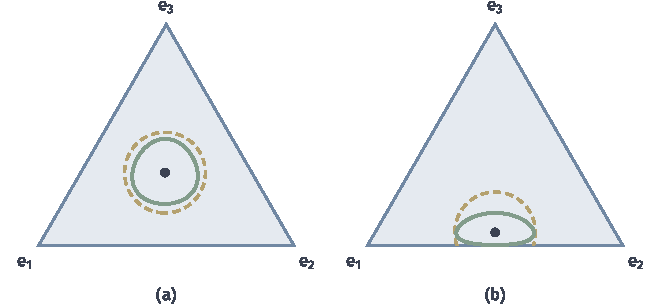
\includegraphics[width=112mm]{figures/05-optimization/06-constrained-optimization/matplotlib/feas-kl-balls/figure.pdf}
  \caption{同一单纯形上两把尺子的等距线。绿色实线是熵势的$\{\bm{u}:D_h(\bm{u},\bm{c})=0.05\}$，黄色虚线是欧氏圆$\{\bm{u}:\tfrac12\lVert\bm{u}-\bm{c}\rVert_2^2=0.025\}$，黑点是中心$\bm{c}$。(a)$\bm{c}\approx(1/3,1/3,1/3)$。(b)$\bm{c}=(0.47,0.47,0.06)$，靠近底边，绿色曲线在朝边的一侧被压扁，黄色圆已越出三角形。}
  \label{fig:feas-kl-balls}
\end{BookInlineFigure}

\subsection{镜像更新}
\label{sec:feas-mirror-update}

有了新尺子，更新公式是什么？它又如何退回熟悉的投影梯度？

\paragraph{主要思想}
投影梯度在$\bm{C}$上最小化线性模型加欧氏距离。把欧氏距离换成$D_h$，就得到\term{镜像下降法}（mirror descent）\scite{beck2003mirror}：
\begin{equation}
 \bm{x}^{(t+1)}\in\argmin_{\bm{x}\in\bm{C}}\Bigl\{\alpha^{(t)}\langle\bm{g}^{(t)},\bm{x}\rangle+D_h(\bm{x},\bm{x}^{(t)})\Bigr\}.
 \label{eq:feas-mirror}
\end{equation}
这里$\bm{g}^{(t)}$可以是当前梯度，也可以是目标非光滑时所选的一个凸次梯度。次梯度的定义见第~\ref{chap:nonsmooth-composite-optimization}章。

$D_h$的作用相当于一根弹簧，把新点拉住，不让它离当前点太远。不同的是，这根弹簧的松紧随位置变化。

\paragraph{完整的计算}
式~\eqref{eq:feas-mirror}可以拆成三步。设$\bm{C}$在$h$的可微区域内，先对$\bm{x}$求驻点。$D_h(\bm{x},\bm{x}^{(t)})$关于$\bm{x}$的梯度是$\nabla h(\bm{x})-\nabla h(\bm{x}^{(t)})$，于是无约束时的驻点$\bm{w}$满足
\begin{equation}
 \nabla h(\bm{w})=\nabla h(\bm{x}^{(t)})-\alpha^{(t)}\bm{g}^{(t)}.
 \label{eq:feas-mirror-dual}
\end{equation}

这说明梯度步不是在变量本身上走，而是在$\nabla h$的值上走。第一步，用$\nabla h$把$\bm{x}^{(t)}$映到梯度空间。第二步，在那里减去$\alpha^{(t)}\bm{g}^{(t)}$。第三步，用$\nabla h$的逆映射取回变量空间，得到$\bm{w}$。

$\bm{w}$可能不在$\bm{C}$中。把式~\eqref{eq:feas-mirror}的目标用式~\eqref{eq:feas-mirror-dual}改写，常数项不影响最小点，于是
\[
 \bm{x}^{(t+1)}=\argmin_{\bm{x}\in\bm{C}}D_h(\bm{x},\bm{w}).
\]
这是按$D_h$度量的投影。图~\ref{fig:feas-mirror-map}把这个往返过程画了出来，“镜像”这个名字指的就是$\nabla h$在两个空间之间的来回映射。

\begin{BookInlineFigure}
  \centering
  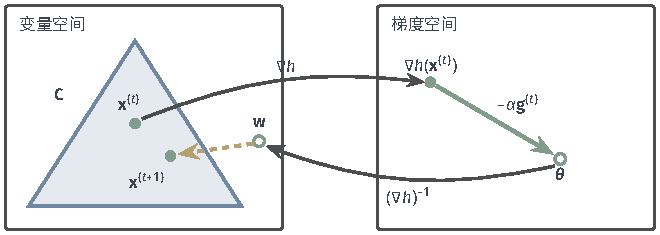
\includegraphics[width=111.74mm]{figures/05-optimization/06-constrained-optimization/tikz/feas-mirror-map/figure.pdf}
  \caption{镜像更新的结构。$\nabla h$把当前点送到梯度空间，绿色箭头在那里减去$\alpha\bm{g}^{(t)}$，逆映射把结果带回变量空间得到$\bm{w}$，黄色虚线按$D_h$投影回集合$\bm{C}$得到$\bm{x}^{(t+1)}$。}
  \label{fig:feas-mirror-map}
\end{BookInlineFigure}

取$h=\tfrac12\lVert\cdot\rVert_2^2$，$\nabla h$是恒等映射，式~\eqref{eq:feas-mirror-dual}给出$\bm{w}=\bm{x}^{(t)}-\alpha^{(t)}\bm{g}^{(t)}$，再做欧氏投影，正是式~\eqref{eq:feas-pgd}。所以投影梯度是镜像下降的特例。

\paragraph{其他势函数要核对的事}
换一个势函数，要分别回答三个问题。解是否存在：若$\bm{C}$紧、$h$连续，子问题有解；否则要检查水平集。解是否唯一：$h$严格凸时唯一。下一步能否继续：$\bm{x}^{(t+1)}$必须落在$h$的可微区域内，否则$\nabla h(\bm{x}^{(t+1)})$不存在，式~\eqref{eq:feas-bregman}无法展开。

第三个问题最容易被忽略。以一元势函数$h(x)=x^{3/2}$（定义域$x\geq0$）为例，导数$\tfrac32\sqrt{x}$在边界保持有限，梯度为正且步长足够大时，子问题的解就落在$x=0$上。这个点在定义域的边界，$h$作为定义域外取$+\infty$的函数在此处不可微。熵势不会发生这种事：它的导数在边界趋于$-\infty$，下一小节会看到迭代被挡在内部。

\subsection{熵势与指数更新}
\label{sec:feas-entropy}

单纯形上的比例变量适合用哪只碗？用\term{熵势}（entropic potential）可以把式~\eqref{eq:feas-mirror}解成闭式，并得到乘法形式的更新。

\paragraph{熵势}
取
\begin{equation}
 h(\bm{x})=\sum_{i=1}^nx_i\ln x_i,\qquad\bm{x}\geq\bm{0},
 \label{eq:feas-entropy}
\end{equation}
并按$0\ln0=0$延拓到坐标为零的边界。$h$在$\bm{x}\geq\bm{0}$上连续，梯度$\nabla h(\bm{x})_i=\ln x_i+1$只在所有坐标为正时存在，所以展开点必须是正向量。

对坐标和都为一的$\bm{u}$和正向量$\bm{x}$，代入式~\eqref{eq:feas-bregman}，线性项中的$\sum_i(u_i-x_i)$等于零，得到
\begin{equation}
 D_h(\bm{u},\bm{x})=\sum_{i=1}^nu_i\ln\frac{u_i}{x_i}.
 \label{eq:feas-kl}
\end{equation}

\paragraph{指数更新}
在$\bm{\Delta}$上解式~\eqref{eq:feas-mirror}。从正向量$\bm{x}^{(t)}$出发，暂时忽略$\bm{x}\geq\bm{0}$，只对等式约束引入乘子$\nu$，对$x_i$求偏导并令其为零：
\[
 \alpha g_i+\ln\frac{x_i}{x_i^{(t)}}+1+\nu=0.
\]

解出$x_i$，常数因子$\mathrm{e}^{-1-\nu}$对所有坐标相同，它由坐标和为一确定，于是
\begin{equation}
 x_i^{(t+1)}=\frac{x_i^{(t)}\exp\bigl(-\alpha g_i\bigr)}{\sum_{j=1}^nx_j^{(t)}\exp\bigl(-\alpha g_j\bigr)}.
 \label{eq:feas-exponential}
\end{equation}

结果每个坐标严格为正，所以被忽略的约束$\bm{x}\geq\bm{0}$确实不活跃，上面的驻点是原子问题的解（目标严格凸，驻点唯一）。下一步的展开点仍是正向量，迭代可以无限进行下去。这种\term{指数更新}（exponentiated update）是乘法的：梯度小的坐标放大，梯度大的坐标缩小，最后归一化。

\paragraph{两个坐标的比较}
设只有两个坐标，$\bm{x}=(0.9,0.1)$，$\bm{g}=(0,1)$，$\alpha=\tfrac12$。投影梯度的梯度步终点是$(0.9,-0.4)$，投影到线段上得到
\[
 \bm{x}^{+}_{\text{投影}}=(1,0).
\]

指数更新先算$(0.9,\;0.1\mathrm{e}^{-1/2})=(0.9,\;0.06065)$，归一化得
\[
 \bm{x}^{+}_{\text{镜像}}\approx(0.9369,0.0631).
\]
投影梯度一步把第二个坐标截到零，镜像更新只把它减小了约$37\%$。

两者的差别随坐标大小变化。两个坐标时投影更新是$x_2^{+}=\max\{x_2-\tfrac12\alpha(g_2-g_1),0\}$，变化量与$x_2$本身无关；镜像更新是乘以一个因子。图~\ref{fig:feas-exp-vs-proj}显示：$x_2=0.5$时两者起步斜率相同；$x_2=0.05$时投影很快归零，镜像更新则按比例缓慢减小。

\begin{BookInlineFigure}
  \centering
  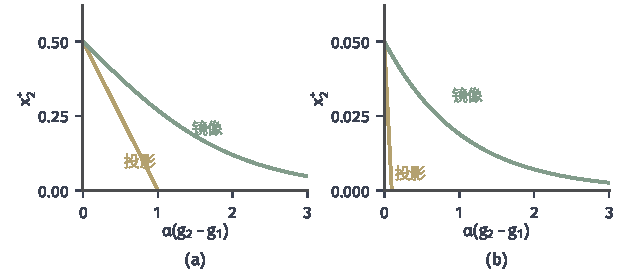
\includegraphics[width=108mm]{figures/05-optimization/06-constrained-optimization/matplotlib/feas-exp-vs-proj/figure.pdf}
  \caption{两个坐标的一步更新，横轴是梯度差乘步长，纵轴是新的$x_2$。黄线是投影更新，绿线是指数更新。(a)$x_2=0.5$，$x_2$较大时两者在起点相切。(b)$x_2=0.05$，投影在横轴$0.1$处归零，指数更新缓慢衰减。}
  \label{fig:feas-exp-vs-proj}
\end{BookInlineFigure}

\needspace{6\baselineskip}
\paragraph{变量}
\begin{itemize}
 \item $\bm{x}^{(t)}\in\bm{\Delta}$：当前点，所有坐标为正。
 \item $\bm{g}^{(t)}$：当前梯度或所选次梯度。
 \item $\bm{w}^{(t)}\in\mathbb{R}^n$：归一化前的正向量。
 \item $\alpha>0$：步长；$T$：总步数。
\end{itemize}

\paragraph{初始化}
取正向量起点，常用均匀分布。例中与投影梯度用同一起点$\bm{x}^{(0)}=(0.1,0.2,0.7)$，步长$\alpha=1/4$，第~\ref{sec:feas-mirror-progress}节说明这个步长的来历。

\needspace{6\baselineskip}
\paragraph{每轮更新}
在第$t$轮：
\begin{enumerate}
 \item \textbf{计算指数因子。}每个坐标乘以指数因子，得到$\bm{w}^{(t)}$。例中第一轮$\bm{g}^{(0)}=(-0.9,-1.7,1.4)$，于是
 \[
  \bm{w}^{(0)}\approx(0.12523,0.30592,0.49328).
 \]
 \item \textbf{归一化。}由式~\eqref{eq:feas-exponential}，把$\bm{w}^{(t)}$除以坐标和得到$\bm{x}^{(t+1)}$。例中第一轮分母约为$0.92443$，于是
 \[
  \bm{x}^{(1)}\approx(0.13547,0.33093,0.53361),\qquad f(\bm{x}^{(1)})\approx0.83140.
 \]
\end{enumerate}

例中第二轮$\bm{g}^{(1)}\approx(-0.8645,-1.1763,1.0672)$，分母约为$1.02087$，于是
\[
 \bm{x}^{(2)}\approx(0.16472,0.43499,0.40030),\qquad f(\bm{x}^{(2)})\approx0.58130.
\]

例中第三轮$\bm{g}^{(2)}\approx(-0.8353,-0.7601,0.8006)$，分母约为$1.05667$，于是
\[
 \bm{x}^{(3)}\approx(0.19208,0.49781,0.31011),\qquad f(\bm{x}^{(3)})\approx0.45489.
\]

运行到$T=60$，目标差约为$6.6\times10^{-5}$，第三个坐标始终为正。最终得到的$\bm{x}^{(60)}$在$x_3$上还有约$1.3\times10^{-4}$的残留量，它每轮大约乘以$0.88$，但不会精确到零。

图~\ref{fig:feas-md-path}将它和投影梯度比较。投影梯度在第$3$步把$x_3$截成零，之后活动集就固定了。镜像下降的路径光滑，$x_3$每轮大约乘以同一个因子。这是一种取舍：投影能识别出活动约束，镜像更新保持稠密的正权重。

\begin{BookInlineFigure}
  \centering
  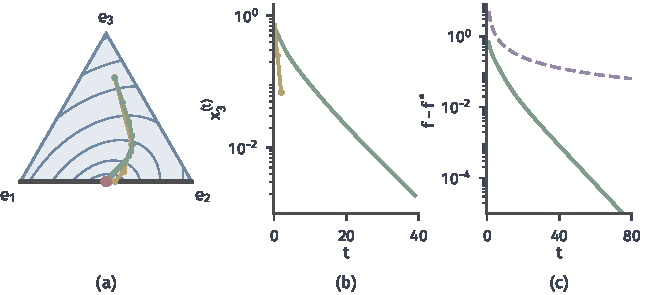
\includegraphics[width=112mm]{figures/05-optimization/06-constrained-optimization/matplotlib/feas-md-path/figure.pdf}
  \caption{预算例上的镜像下降（绿）与投影梯度（黄），步长都是$1/4$，起点$(0.1,0.2,0.7)$。(a)两条路径，镜像下降的路径弯曲着逼近底边。(b)第三个坐标$x_3^{(t)}$（对数轴）：投影梯度第$3$步起为零，从图中消失；镜像下降几何衰减。(c)镜像下降的目标差（绿）与定理~\ref{thm:feas-mirror-smooth}的上界$LD_h(\bm{x}^\star,\bm{x}^{(0)})/T$（紫色虚线）。}
  \label{fig:feas-md-path}
\end{BookInlineFigure}

\subsection{进展与输出}
\label{sec:feas-mirror-progress}

镜像下降的一次更新到底带来了多少进展？目标是否一定下降？答案取决于手上有哪种假设。

\paragraph{三点关系}
分析的工具是下面的引理，它把一次更新转成比较点到两个迭代点的$D_h$之差，求和时可以裂项。

\begin{lemma}[三点关系]
\label{lem:feas-three-point}
设$\bm{C}$闭凸，$h$在开集$\bm{U}$上可微且凸，$\bm{x}\in\bm{U}$，$\bm{x}^{+}$是式~\eqref{eq:feas-mirror}的解，并且$\bm{x}^{+}\in\bm{U}$。则对所有$\bm{u}\in\bm{C}\cap\operatorname{dom}h$，
\begin{equation}
 \alpha\langle\bm{g},\bm{x}^{+}-\bm{u}\rangle\leq D_h(\bm{u},\bm{x})-D_h(\bm{u},\bm{x}^{+})-D_h(\bm{x}^{+},\bm{x}).
 \label{eq:feas-three-point}
\end{equation}
\end{lemma}

\begin{proof}
式~\eqref{eq:feas-mirror}是凸目标在凸集上的最小化，$\bm{x}^{+}$满足变分不等式：
\[
 \bigl\langle\alpha\bm{g}+\nabla h(\bm{x}^{+})-\nabla h(\bm{x}),\ \bm{u}-\bm{x}^{+}\bigr\rangle\geq0.
\]

移项得到
\[
 \alpha\langle\bm{g},\bm{x}^{+}-\bm{u}\rangle\leq\bigl\langle\nabla h(\bm{x}^{+})-\nabla h(\bm{x}),\ \bm{u}-\bm{x}^{+}\bigr\rangle.
\]

把式~\eqref{eq:feas-bregman}的三个距离展开相减，$h(\bm{u})$、$h(\bm{x})$、$h(\bm{x}^{+})$都抵消，剩下的线性项正好是
\[
 D_h(\bm{u},\bm{x})-D_h(\bm{u},\bm{x}^{+})-D_h(\bm{x}^{+},\bm{x})
 =\bigl\langle\nabla h(\bm{x}^{+})-\nabla h(\bm{x}),\ \bm{u}-\bm{x}^{+}\bigr\rangle.
\]
代入上式即得结论。
\end{proof}

\paragraph{次梯度分析}
第一种情形只假设次梯度有界，目标可以不光滑。设$\lVert\cdot\rVert$是某个范数，它的对偶范数是
\[
 \lVert\bm{g}\rVert_{*}=\max_{\lVert\bm{v}\rVert\leq1}\langle\bm{g},\bm{v}\rangle.
\]

\begin{theorem}[镜像下降的平均点界]
\label{thm:feas-mirror-subgrad}
设$\bm{C}$闭凸，$f$在$\bm{C}$上凸，$\bm{g}^{(t)}$是$f$在$\bm{x}^{(t)}$处的次梯度，$\lVert\bm{g}^{(t)}\rVert_{*}\leq G$。设各迭代点都在$h$的可微区域内，且在$\bm{C}$上
\begin{equation}
 D_h(\bm{u},\bm{x})\geq\tfrac12\lVert\bm{u}-\bm{x}\rVert^2.
 \label{eq:feas-h-strong}
\end{equation}
取固定步长$\alpha$，平均点$\bar{\bm{x}}=\frac1T\sum_{t<T}\bm{x}^{(t)}$，则对$\bm{u}\in\bm{C}$，
\begin{equation}
 f(\bar{\bm{x}})-f(\bm{u})\leq\frac{D_h(\bm{u},\bm{x}^{(0)})}{\alpha T}+\frac{\alpha G^2}{2}.
 \label{eq:feas-mirror-rate}
\end{equation}
\end{theorem}

\begin{proof}
记$\bm{x}=\bm{x}^{(t)}$，$\bm{x}^{+}=\bm{x}^{(t+1)}$，$\bm{g}=\bm{g}^{(t)}$。由次梯度不等式，把内积拆成两部分：
\[
 \alpha\bigl(f(\bm{x})-f(\bm{u})\bigr)\leq\alpha\langle\bm{g},\bm{x}^{+}-\bm{u}\rangle+\alpha\langle\bm{g},\bm{x}-\bm{x}^{+}\rangle.
\]

第二项用对偶范数和Young不等式放大，再用$D_h$的强凸下界：
\[
 \alpha\langle\bm{g},\bm{x}-\bm{x}^{+}\rangle\leq\frac{\alpha^2G^2}{2}+\frac12\lVert\bm{x}-\bm{x}^{+}\rVert^2\leq\frac{\alpha^2G^2}{2}+D_h(\bm{x}^{+},\bm{x}).
\]

第一项用引理~\ref{lem:feas-three-point}，$D_h(\bm{x}^{+},\bm{x})$恰好抵消，得到
\[
 \alpha\bigl(f(\bm{x}^{(t)})-f(\bm{u})\bigr)\leq D_h(\bm{u},\bm{x}^{(t)})-D_h(\bm{u},\bm{x}^{(t+1)})+\frac{\alpha^2G^2}{2}.
\]

对$t=0,\ldots,T-1$求和，右端裂项，丢掉末项$D_h\geq0$。两边除以$\alpha T$，再用$f$的凸性把平均值换成$f(\bar{\bm{x}})$，即得结论。
\end{proof}

\paragraph{熵势给出的常数}
在单纯形上，取$\lVert\cdot\rVert=\lVert\cdot\rVert_1$，对偶范数是$\lVert\cdot\rVert_\infty$。熵势满足定理的强凸条件。设$\bm{v}=\bm{u}-\bm{x}$，$\bm{w}$是线段上任一点，$\nabla^2h(\bm{w})=\operatorname{diag}(1/w_i)$，由Cauchy--Schwarz不等式和$\sum_iw_i=1$，
\[
 \bm{v}^\top\nabla^2h(\bm{w})\bm{v}=\sum_i\frac{v_i^2}{w_i}\geq\frac{(\sum_i\lvert v_i\rvert)^2}{\sum_iw_i}=\lVert\bm{v}\rVert_1^2.
\]
由Taylor公式的积分余项，这给出式~\eqref{eq:feas-h-strong}，范数取$\lVert\cdot\rVert_1$。

从均匀分布出发，由式~\eqref{eq:feas-kl}和$\sum_iu_i\ln u_i\leq0$得到$D_h(\bm{u},\bm{x}^{(0)})\leq\ln n$。在式~\eqref{eq:feas-mirror-rate}中取$\alpha=\sqrt{2\ln n/T}/G$，得到
\begin{equation}
 f(\bar{\bm{x}})-f^\star\leq G\sqrt{\frac{2\ln n}{T}},\qquad\lVert\bm{g}^{(t)}\rVert_\infty\leq G.
 \label{eq:feas-entropy-rate}
\end{equation}

投影次梯度法对同一问题的上界要用$\lVert\bm{g}\rVert_2$，而$\lVert\bm{g}\rVert_2$可以大到$\sqrt{n}\,G$。所以梯度稠密时，熵势的上界在维数依赖上小了约$\sqrt{n/\ln n}$倍。这是两个上界的比较，并不保证熵势在每个问题上都更快。

\paragraph{光滑性带来的下降}
第二种情形假设$f$相对于$h$光滑，即存在$L>0$，使$Lh-f$在$\bm{C}$上凸。把凸性写成切平面不等式，它等价于
\begin{equation}
 f(\bm{u})\leq f(\bm{x})+\langle\nabla f(\bm{x}),\bm{u}-\bm{x}\rangle+LD_h(\bm{u},\bm{x}),
 \label{eq:feas-relative-smooth}
\end{equation}
称为\term{相对光滑}（relative smoothness）。$h=\tfrac12\lVert\cdot\rVert_2^2$时它就是下降引理。

预算例满足这个条件。单纯形上$x_i\leq1$，由此
\[
 \bm{v}^\top\nabla^2f\,\bm{v}\leq4\lVert\bm{v}\rVert_2^2\leq4\sum_i\frac{v_i^2}{x_i}=4\,\bm{v}^\top\nabla^2h\,\bm{v},
\]
所以$L=4$可用，这正是取$\alpha=1/4$的依据。

\begin{theorem}[相对光滑下的镜像下降]
\label{thm:feas-mirror-smooth}
设$f$凸可微，满足式~\eqref{eq:feas-relative-smooth}，各迭代点在$h$的可微区域内，取$\alpha=1/L$。则目标逐步下降，
\begin{equation}
 f(\bm{x}^{(t+1)})\leq f(\bm{x}^{(t)})-LD_h(\bm{x}^{(t)},\bm{x}^{(t+1)}),
 \label{eq:feas-mirror-descent}
\end{equation}
并且对$\bm{u}\in\bm{C}$，
\begin{equation}
 f(\bm{x}^{(T)})-f(\bm{u})\leq\frac{LD_h(\bm{u},\bm{x}^{(0)})}{T}.
 \label{eq:feas-mirror-smooth-rate}
\end{equation}
\end{theorem}

\begin{proof}
记$\bm{x}=\bm{x}^{(t)}$，$\bm{x}^{+}=\bm{x}^{(t+1)}$，$\bm{g}=\nabla f(\bm{x})$。由式~\eqref{eq:feas-relative-smooth}，
\[
 f(\bm{x}^{+})\leq f(\bm{x})+\langle\bm{g},\bm{x}^{+}-\bm{x}\rangle+LD_h(\bm{x}^{+},\bm{x}).
\]

在式~\eqref{eq:feas-three-point}中取$\alpha=1/L$，$\bm{u}=\bm{x}$，并用$D_h(\bm{x},\bm{x})=0$，得到
\[
 \langle\bm{g},\bm{x}^{+}-\bm{x}\rangle+LD_h(\bm{x}^{+},\bm{x})\leq-LD_h(\bm{x},\bm{x}^{+}).
\]
两式合起来就是下降式。

再用凸性给出的切平面下界$f(\bm{u})\geq f(\bm{x})+\cdots$，与上面第一式相减，得到
\[
 f(\bm{x}^{+})-f(\bm{u})\leq\langle\bm{g},\bm{x}^{+}-\bm{u}\rangle+LD_h(\bm{x}^{+},\bm{x}).
\]

用式~\eqref{eq:feas-three-point}，右端不超过$L\bigl[D_h(\bm{u},\bm{x})-D_h(\bm{u},\bm{x}^{+})\bigr]$。对$t$求和裂项，再由目标单调，最后一项不超过平均值，即得结论。
\end{proof}

预算例中$D_h(\bm{x}^\star,\bm{x}^{(0)})\approx1.263$，$L=4$，上界约为$5.05/T$，$T=60$时约为$0.084$，实际目标差约$6.6\times10^{-5}$。

\paragraph{目标不一定下降}
定理~\ref{thm:feas-mirror-subgrad}只保证平均点，不保证目标逐步下降，下面的例子说明这是真实的。在$\bm{\Delta}\subset\mathbb{R}^2$上取$f(\bm{x})=\lvert x_1-x_2\rvert$，$\bm{x}=(0.6,0.4)$，次梯度$\bm{g}=(1,-1)$，$\alpha=1$。由式~\eqref{eq:feas-exponential}，
\[
 \bm{x}^{+}\approx(0.1687,0.8313),\qquad f(\bm{x}^{+})\approx0.6626.
\]
目标从$0.2$升到了$0.6626$。次梯度步在不光滑的折点附近可以越过很远，所以输出时应使用平均点，或记录迄今最好的点。表~\ref{tab:feas-mirror-cases}对比了两种分析。

\begin{BookInlineTable}
  \centering
  \caption{镜像下降的两种分析。}
  \label{tab:feas-mirror-cases}
  \begin{tabular}{lll}
   \toprule
   & 次梯度分析 & 相对光滑分析\\
   \midrule
   目标 & 凸，可不光滑 & 凸，相对光滑\\
   势函数 & 按范数强凸 & $Lh-f$凸\\
   步长 & 依$T$或递减 & $1/L$\\
   目标值单调 & 否 & 是\\
   输出 & 平均点 & 最后一点\\
   上界的阶 & $1/\sqrt{T}$ & $1/T$\\
   \bottomrule
  \end{tabular}
\end{BookInlineTable}
